\documentclass[9pt,twocolumn,twoside]{cidlab-draft}

\templatetype{cidlab-invited}

\title{Bayesian inference and testing any hypothesis you can
specify}

\usepackage{
	amsmath,amssymb,amsfonts,
    csquotes,
	epsfig,epstopdf,epigraph,
    graphicx,
    mathtools,
	subfig,
    tikz,
    url}
\usepackage[super]{nth}
\usepackage[english]{babel}
\usepackage[]{todonotes}
\usepackage[many]{tcolorbox}
\usepackage{setspace}

\definecolor{BurntOrange}{rgb}{0.8,0.4,0.0}
\newcommand{\hyp}[1]{{\color{BurntOrange}{#1}}}

\newtcolorbox{framefloat}[1][!tb]{arc=5pt,outer arc=5pt,boxrule=0.4pt,float*=t,
  colframe=black,colback=BurntOrange,float=#1}
\tcbset{float*=t,width=\textwidth,colback=orange!10!white,colframe=orange!80!black,enhanced}

\renewcommand{\H}{{\mathcal{H}}}
\renewcommand{\:}{{:}}

\newcommand{\osf}{\url{https://osf.io/mvp53/}}
\newcommand{\jv}[1]{\todo[color=orange,inline]{#1}}

\newcommand{\bino}[1]{\binom{n}{k} #1^k (1-#1)^{n-k}}
\newcommand*\diff{\mathop{}\!\mathrm{d}}

\newcommand{\red}[1]{{\color{red}#1}}

\author[a]{Alexander Etz}
\author[b]{Julia M.\ Haaf}
\author[a,b]{Jeffrey N.\ Rouder}
\author[a,$\dagger$]{Joachim Vandekerckhove}

\affil[a]{University of California, Irvine}
\affil[b]{University of Missouri}

\leadauthor{Etz} 

\significancestatement{}
\authorcontributions{}
\equalauthors{}
\authordeclaration{The authors declare no conflicts of interest. The authors were supported by National Science Foundation grant \#1534472 to JV and the National Science Foundation Graduate Research Fellowship Program \#DGE-1321846 to AE.}
\correspondingauthor{\textsuperscript{$\dagger$}To whom correspondence should be addressed. E-mail: joachim@uci.edu.}

\keywords{Bayesian inference $|$ Bayesian statistics $|$ Bayes factor $|$ Testing the null $|$ Philosophy of science} 

\begin{abstract} 
Hypothesis testing is a special form of model selection.  Once a pair of competing models is fully defined, their definition immediately leads to a measure of how strongly each model supports the data.  The ratio of their support is often called the likelihood ratio or the Bayes factor.  Critical in the model selection endeavor is the specification of the models.  In the case of hypothesis testing, it is of the greatest importance that we specify exactly what is meant by a ``null'' hypothesis as well as the alternative to which it is contrasted, and that these are suitable instantiations of theoretical positions.  Here, we provide an overview of different instantiations of null and alternative hypotheses that can be useful in practice, while the underlying method of likelihood comparison is universal and identical in all cases.  An associated app can be found via \osf{}.
\end{abstract}

\dates{This manuscript was compiled on \today}

\graphicspath{{./pics/}}

\begin{document}

\thispagestyle{firststyle}

\maketitle

\epigraph{Just as a computer stands ready to perform any calculation we ask of it, our present theory of Bayesian inference stands ready to answer any question we put to it.}{E.\ T.\ Jaynes \protect\cite[p.~382]{rosenkrantz1983jaynes}}

\noindent The topic of this special section of \emph{Advances in Methods and Practices in Psychological Science} is ``providing evidence against a (meaningful) effect.''  Here, we will provide a few examples of how such evidence can be quantified.  Once evidence is quantified, it can easily be combined with existing knowledge to evaluate the probability that an effect is (practically) non-existent.

However, owing to the advancement of statistical computing power, it is not the \textit{computation} of evidence or of probabilities that is most challenging in scientific inference. What is critical in the evaluation of theories, models, and hypotheses is that they are \emph{clearly} and \emph{unambiguously} specified. Indeed, once a model is sufficiently specified, the scientist only has to ``turn the crank'' of inference to calculate the evidence for or against some theory \cite{edwards1963bayesian}. Both for the quantification of evidence and for combining evidence with prior knowledge, we can turn to probability theory.  The use of probability theory for this goal starts with \citeA{Bayes:1763}, and is followed by seminal advances due to \citeA{deFinetti:1974}, \citeA{Jeffreys1961}, \citeA{Laplace:1829}, and \citeA{Savage:1951}.  Several tutorials in the psychological literature are available including our most recent ones \citeA{EtzSI} and \citeA{Rouder:Morey:inpress}.

Here, we provide a theoretical introduction to the step that precedes these computational steps: stating a question clearly. We illustrate how slightly different questions can lead to different outcomes, and how models that seem qualitatively different are sometimes very difficult to distinguish. 
In order to set up our discussion of precise scientific hypotheses, we first introduce some relevant concepts from the philosophy of science and statistics.

\paragraph{Occam's Razor and Russell's Teapot}
It is hopefully self-evident that no statistical procedure can discriminate between two models if they make exactly the same predictions for all scenarios \cite{WrinchJeffreys1921}. Similarly, if one of the models is so flexible that it generates predictions that are \emph{arbitrarily close} to the predictions of the other, they can strictly speaking not be distinguished. For example, if Theory~A says that some difference is 0 IQ points, Theory~B says the difference is 10$^{-12}$ IQ points, and modern studies have a maximum precision of roughly 5 points of difference, then intelligence researchers will simply have to make peace with the fact that these two theories cannot be told apart from IQ data alone. If, on the other hand, Theory~C says that the difference can be anywhere from -100 to +100, \emph{and the available data happen to indicate that the difference is very close to zero}, we are justified in concluding that the more complex, less parsimonious Theory~C should probably be discarded.

A famous argument by Bertrand Russell \citeyear{russell1952there} involves a mysterious teapot orbiting the Sun, somewhere between Earth and the planet Mars. To summarize the argument: no observations that we have available can conclusively rule out the existence of such a teapot -- the ``teapot theory'' and the ``no teapot theory'' make essentially identical predictions about the data received by even the strongest of our telescopes.\footnote{And should the authors be wrong on this account, the celestial teapot can easily be amended to be sentient, timid, and having the ability to make itself invisible.} However, the litany of additional assumptions that one would need in order to make the celestial teapot theory likely is so extensive that any rational observer (justly) rejects the claim out of hand. The theory is not per se falsified by any data, but it lacks parsimony, and so with each observation that fails to confirm the existence of the teapot, evidence for its nonexistence accrues. Figure~\ref{fig:xkcd} provides a modern example of the same line of reasoning.  This concept---that all other things being equal, simpler theories are preferred to more complex theories---is alternatively known as Occam's razor, the principle of parsimony, and the simplicity rule \cite{Myung:Pitt:1997,VandekerckhoveEtAl2015MPT}.

\begin{figure}[bt]
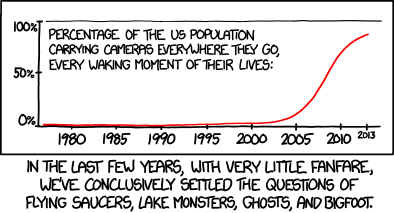
\includegraphics[width=.475\textwidth]{settled.png}
\caption{The existence of a number of unlikely creatures such as lake monsters and the sasquatch has gradually become falsified over the last decade or so as mobile cameras have become ubiquitous.  The implication is that, if such creatures did exist, clear photographic evidence would be available by now with high probability.  By contrast, if they did not exist, any photographic evidence would be unclear and unconvincing as it always has been. Since clearer photographs have not emerged, and there are no strong prior reasons to believe in these phenomena, we may reasonably conclude that lake monsters, flying saucers, ghosts, and Bigfoot do not exist. However, the jury is still out on the Grinch, Whos, and other snowflake-dwellers. This drawing is titled ``Settled'' and is \copyright Randall Munroe (xkcd.com/1235).
}\label{fig:xkcd}
\end{figure}

Both of these insights---that some theories are impossible or impractical to distinguish from one another and that the more parsimonious explanation is preferable---from the philosophy of science are independently codified by probability theory, as we will demonstrate.

\paragraph{Jeffreys's Platitude} As cell phone cameras have become more ubiquitous, the likelihood that Bigfoot exists has gradually dwindled.  Similarly, as telescopes grow more and more powerful, we gradually falsify the existence of Russell's Teapot.  However, an important realization in falsifying the existence of some phenomenon is that the ``mere existence'' hypothesis is often underspecified.  Suppose, for example, that Russell had specified that his teapot is approximately the size of Mars, and that it always resides close to the red planet.  This particularisation of the teapot theory, while valid, is clearly falsified by the available data (because such an object would be visible to the naked eye).  There is a clear distinction between the questions ``Does the celestial teapot exist?'' and ``Does a celestial teapot with a volume of about 1.6 $\times$ 10\textsuperscript{11} km\textsuperscript{3} exist?''

Jeffreys's Platitude \cite{Jeffreys1939} is, to paraphrase slightly, ``Answers depend on questions.'' In the context of statistical testing, it should be a platitude that if we change the definition of a statistical model (including changes in the prior knowledge regarding which values parameters can and do take; such as the supposed volume of a teapot), it should not come as a surprise that the evidence for or against this model may change as a result.

\paragraph{Statistical inference} 
We have stressed above that the crux of inference is formulating the scientific question of primary interest. We then must construct a statistical model to represent our scientific problem and identify the quantities of interest (e.g., what represents a ``meaningful'' or ``practically relevant'' effect?), before seeing how our data inform the probability of these quantities. Within the framework of Bayesian inference this process is essentially automatic, following naturally from probability theory and using Bayes' theorem in particular. 

We will not go into the finer details here (see \citeNP{kass1995bayes}) except to point out that the probabilistic framework is used to update the prior probability of a theory (i.e., its plausibility before the data are seen) into its posterior probability (after the data are seen). The change in the relative probability of any two models after seeing the data is captured by the Bayes factor \cite{Jeffreys1961}. Specifically, we multiply the prior odds in favor of a meaningful effect with the Bayes factor ($B$) to obtain the posterior odds in favor of that effect:
$$
\underbrace{\frac{P(\text{meaningful effect})}{P(\text{no meaningful effect})}}_\text{odds before seeing the data} \times {B}
=
\underbrace{\frac{P(\text{meaningful effect}|\text{data})}{P(\text{no meaningful effect}|\text{data})}}_\text{odds after seeing the data}
$$ 
where the Bayes factor is
\begin{eqnarray}\label{eq:b}
B = \frac{P(\text{data}|\text{meaningful effect})}{P(\text{data}|\text{no meaningful effect})}.
\end{eqnarray}%
If the Bayes factor is larger than 1, the data increase the odds in favor of the existence of a meaningful effect, and vice-versa.

The Bayes factor acts to update our prior odds in favor of a meaningful effect to the posterior odds in favor of a meaningful effect by comparing the probability the two positions give to the observed data. Below we demonstrate how this can be done across a number of scenarios, where what constitutes a ``meaningful effect'' is determined primarily by context. As a result, it will become clear that there is no such thing as ``the'' unique Bayes factor for any given data set: the Bayes factor expresses a relationship between the available data on the one hand and the question being asked on the other \cite{morey2011bayes}.  As we have argued above in the context of Jeffreys's Platitude, this is both just and proper, and we should 
be highly skeptical of any inferential method that ignores such important context.

\section*{Possible scenarios}

One way of putting Jeffreys' Platitude in context is to draw a distinction between theoretical positions and model instantiations.  A theoretical position is a verbal statement such as ``there is no true effect'' or ``there is some true effect.''   A statistical hypothesis is an instantiation of a theoretical position that is sufficiently precise that \emph{it predicts where the data should occur before they are seen}.  The verbal statement, ``there is some true effect,'' fails this prediction test---one cannot place a probability distribution over where the data are likely to occur.   \citeA{Rouder:etal:2016b} note that there are often many ways to instantiate hypotheses such as ``there is no effect'' or ``there is some effect.''  Jeffreys' Platitude reminds us that \emph{instantiations matter}.  \citeA{Rouder:etal:2016b} explore this important observation by positing that several research teams might instantiate different effect models.  Here we expand their approach to include different effect and null-effect models.

Once competing models have been carefully constructed, we can activate the Bayesian machinery that allows us to determine how much evidence there is for each account. As has been argued elsewhere (e.g., \citeNP{Cox:1946}, \citeNP{jaynes2003probability}), probability theory is not merely one way of doing this, but indeed it is \textit{uniquely} suited. {The problem of assigning plausibility to competing hypotheses is solved {exclusively} by probability theory}.

\paragraph{The point null hypothesis} 

Consider the popular example of ``feeling the future'' \cite{Bem2011}.  The case of extrasensory perception (ESP) is such that we have very specific hypotheses about what its nonexistence would look like.  If ESP does not exist, \emph{there isn't a smidgen of it}. Performance at a chance task is at chance. The null hypothesis that accurately captures this account is a \hyp{point null hypothesis}. Under this hypothesis the accuracy $\theta$ (theta) at a guessing task with two alternatives is exactly one-half. This hypothesis is visualized in Figure~\ref{fig:pv} (top) as a spike distribution (i.e., a vertical line). 

What remains is to define an appropriate alternative to which this point hypothesis is to be compared.  Here we run into what we might call a \emph{teapot problem}: Any amount of ESP would be a discovery for the ages but, much like the trepid teapot or the tiny difference in IQ, it is impossible to devise a test that can detect an arbitrarily small deviation in $\theta$. We rapidly reach the theoretical limits of inference. Now what?

One way to address this issue is to thoughtfully craft an alternative theoretical account informed by the specific context of the problem. In just the same way we carefully devise a null hypothesis that accurately captures what we think the absence of ESP should look like, we can craft an alternative that captures what ESP \emph{would} look like, \emph{should} it exist.  This brings us to one candidate.

\paragraph{The uniformly positive hypothesis} One possible conception of ESP is that a person who has it outperforms chance to some extent, but all extents are equally likely. Under this alternative hypothesis, all values for the accuracy $\theta$ that exceed one-half are equally plausible, while all other values are ruled out. This \hyp{uniformly positive hypothesis} is shown in Figure~\ref{fig:pv} (top) as a uniform distribution from \textonehalf{} to 1 (dashed line).  

\begin{figure}[tb]
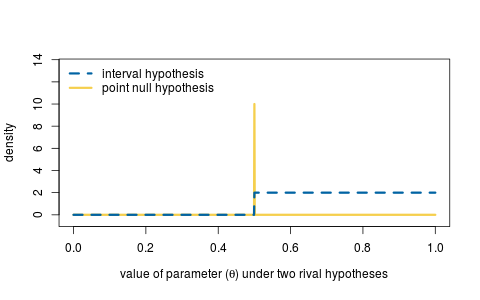
\includegraphics[width=0.49\textwidth]{custom-p.png}\\
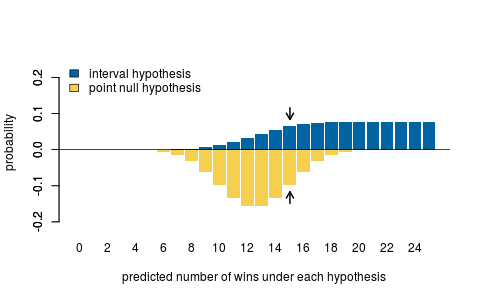
\includegraphics[width=0.49\textwidth]{custom-d.png}
\caption{\textbf{Top.} The point null hypothesis is represented by a spike at \textonehalf{} (solid line), and the uniformly positive alternative spans from \textonehalf{} to 1 (dashed line). \textbf{Bottom.} The predictions from the point null hypothesis (gold, inverted bars) and the uniformly positive alternative (blue). The arrows indicate the observed data in a fictional ESP experiment, and the Bayes factor is the ratio of the heights of the two bars.}\label{fig:pv}
\end{figure}

\section*{The Bayes factor}
Each of the two models now defined---the null hypothesis as a point and the alternative as an interval over one half of the range of possible values---implies a statement about what the data of some experiment would look like if the model were true.  Suppose that we did some experiment on ESP with 25 trials with two choice options.  Under the null, in such an experiment there is approximately a 10\% chance of getting 10 correct responses, 13\% chance of getting 11 correct responses, and so on (Fig.~\ref{fig:pv}, bottom; computations are in Box~2).  Under the alternative, these data outcomes have a probability of only 1\% and 2\%, respectively.  We say that the null ``predicts,'' ``expects,'' or ``supports'' these patterns of data more strongly than does the alternative, but it is important to note that prediction and expectation here are statistical jargon that have, for example, nothing to do with temporal order (i.e., a model can predict or expect observations that have occurred in the past), which is why some of us prefer ``support.''

The inference procedure now proceeds along three steps. First, if possible, determine the prior probability that the null hypothesis is true. For illustrative purposes, let's assume equiprobability: the prior odds are 1:1. Second, use the data to compute the Bayes factor. Third, use the Bayes factor to turn the prior odds into the posterior odds, by multiplying the prior odds with the Bayes factor.

Direct computation of the Bayes factor can be challenging when dealing with complicated models, often requiring numerical approximation, but conceptually it is always \emph{the relative strength with which the observed data were expected under each model}. Suppose, for example, that we observe a participant get 15 correct answers (still out of 25). The point null gives this outcome a 9.74\% probability, while the alternative gives it only 6.43\% (see the darker bar in the bottom panel of Fig.~\ref{fig:pv}), so the Bayes factor is 9.74$/$6.43 = 1.51 in favor of the null. Multiplying 1.51 with the prior odds of 1:1 gives 1.51:1 posterior odds, or a posterior probability on the null hypothesis of just above 60\%.

\section*{Other possible scenarios}

We cannot emphasize enough the importance of Jeffreys's Platitude to the practice of model selection (and hypothesis testing).  For example, here are two other conceptualizations of the presence and absence of ESP that we might consider.

\paragraph{The competing-point hypothesis} 
The simplest bet in a game of American roulette is to pick one color (red or black), which gives winning odds of 18:19, or approximately a 53\% chance of losing.  The 3\% difference is called the house advantage, which is the carefully controlled way in which casinos stack the deck and ensure profit. Suppose that we think that, if ESP exists, it gives a subtle edge to the clairvoyant at roulette -- just enough to match the house advantage (i.e. a 3\% increment). We might now say that this 53\% is the magnitude at which we expect ESP to express itself in our new data. This leads to the most informative alternative possible: an exact specification of the accuracy $\theta$. 

\begin{figure}[tb]
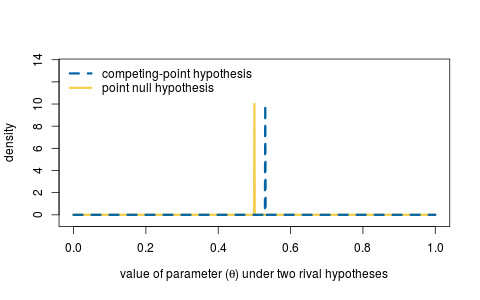
\includegraphics[width=0.49\textwidth]{pointvp-p.png}\\
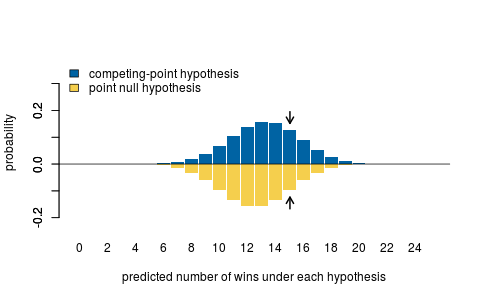
\includegraphics[width=0.49\textwidth]{pointvp-d.png}
\caption{\textbf{Top.} The point null (solid line) and point alternative (dashed line) hypotheses are represented by spikes at 50\% and 53\%, respectively. \textbf{Bottom.} Predictions from the two point hypotheses (point null predictions are drawn in gold and inverted; point alternative predictions in blue) are hard to distinguish, meaning that we will not be able to obtain much evidence for one over the other.}\label{fig:v}
\end{figure}

The \hyp{competing-point hypothesis} is shown in Figure~\ref{fig:v}, with the information about $\theta$ under both hypotheses displayed in the top panel as two spikes, and the associated predictions about the data in the bottom panel as two overlapping histograms.  One salient observation about this scenario is how similar the predictions are.  Even at the very extreme ends of the possible observations (0$/$25 and 25$/$25), the difference in support by the two hypotheses is at most a factor of 4.7.  That is, even the most diagnostic data set of 25 observations imaginable would not deliver very much evidence to discriminate between these two accounts. We have another teapot problem, and would need to gather more data (if we really do care about distinguishing between two so similar hypotheses).

\paragraph{The positive decaying hypothesis} \citeA{rouder2013bayes} instantiated the ``there is some effect'' position by stipulating that, under the ESP hypothesis, people should outperform chance.  The probability of \emph{how much} they do so is not equal: higher performances have lower probabilities, so that 51\% performance is more likely than 52\% and so on.  This is a flexible hypothesis, which allows for all possible values that are greater than chance, but prioritizes small effects over larger ones.  Because they believe this hypothesis made reasonable commitments, \citeA{rouder2013bayes} stressed this \hyp{positive decaying hypothesis} in their meta-analysis of ESP effects.


\paragraph{The negligible-effect hypothesis}
We may also choose different instantiations of the null position.  Another aspect to statistical inference that is often neglected is the \emph{practical significance} of an effect. Suppose that, rather than merely establishing that ESP exists, our goal is to monetize future-telling at a casino -- for example at the roulette table described above.  Once again, in order to reliably outperform the house, a future-teller would have to be at least 53\% accurate.  However, we can be a little more clever about beating the casino, and realize that a future-teller who is reliably \emph{less} than 47\% accurate is also a useful contributor if we simply play the opposite color from their prediction.

Hence, we can formulate a new instantiation of the null that does not, strictly speaking, say that ESP does not exist, merely that its effect is negligible for (our) practical purposes.  Such an hypothesis involves the definition of what is often called an \emph{equivalence region} \cite{Rogers:etal:1993}, and we can test it with exactly the same procedure as before. First, define our smallest non-negligible departure from chance (in this case 3\%), and then define the \hyp{negligible-effect hypothesis}, which states that only values of $\theta$ between $.47$ and $.53$ are plausible (i.e., a region that has a width of 6\%). Next, define a complementary \hyp{non-negligible effect hypothesis}, which consists of two regions: 0 to .47 and .53 to 1.0. 

\begin{figure}[t]
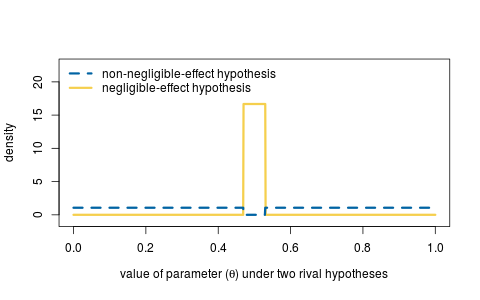
\includegraphics[width=0.49\textwidth]{notched-p.png}\\
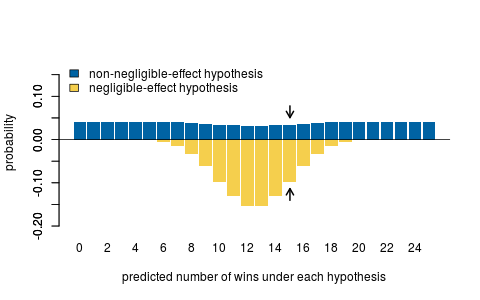
\includegraphics[width=0.49\textwidth]{notched-d.png}
\caption{\textbf{Top.} The solid line represents the null interval (where the effect would be considered negligible) and the dashed line its complement (where the effect is non-negligible). \textbf{Bottom.} Predictions from the two models (predictions from the negligible-effect hypothesis are drawn in gold and inverted; predictions from the complement in blue).}\label{fig:r}
\end{figure}

This comparison is displayed in Figure~\ref{fig:r}. Here we see more clearly an interesting effect that was less obvious in previous applications.  Because the \hyp{non-negligible effect hypothesis} is quite vague---it states that $\theta$ can take any value that is sufficiently far away from 0.5, as in the top panel---and because the total probability that \emph{anything happens} under the hypothesis has to remain exactly 1, the strength of prediction of each individual outcome (bottom panel) is quite low.  That is, to accommodate all the possible outcomes, the model is spread very thin and there is no strong prediction anywhere.

The fact that every model has the same fixed amount of probability to assign to the possible outcomes leads to an automatic penalty for models that hedge over many different possibilities.  This penalty for model freedom is a direct and unavoidable consequence of probability theory, and is a formal implementation of Occam's Razor.

As can be seen in the darker bar in Figure~\ref{fig:r}, the Bayes factor favoring the \hyp{negligible-effect hypothesis} is about 2.8.  If before seeing these data, we held equal prior odds, then now our odds are 2.8:1, or a posterior probability of about 74\% favoring the negligible effect.

\paragraph{The spike and slab comparison} 
Adding to these various null and alternative hypotheses is one particularly common and tempting comparison: as scientists, we will often be interested in knowing if there is \emph{any effect} versus \emph{no effect}.  In so doing, we might wish to forgo specifying any size of effect and simply proclaim that all degrees of non-null accuracy are of interest. This is an ability we have -- we may formulate as null a \hyp{point hypothesis} of no effect (a spike) and as alternative a \hyp{slab hypothesis} that states that all degrees of accuracy are equally plausible (spike-and-slab is a term introduced by \citeNP{mitchell1988})

\begin{figure}[tb]
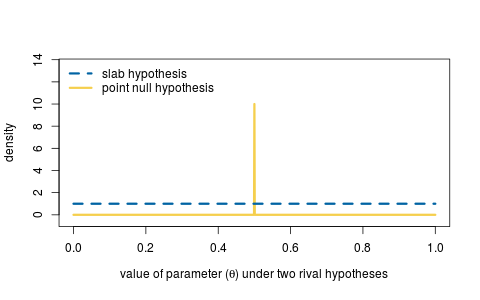
\includegraphics[width=0.49\textwidth]{point-p.png}\\
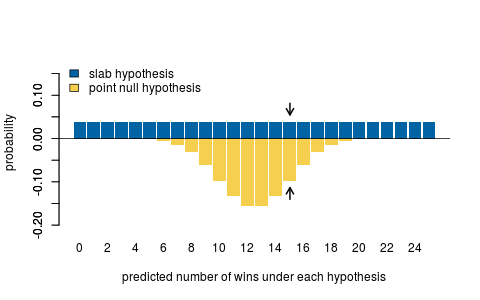
\includegraphics[width=0.49\textwidth]{point-d.png}
\caption{\textbf{Top.} The solid spike represents the point null and the dashed line the alternative. \textbf{Bottom.} The predictions from the two models. Note how similar the predictions of the slab hypothesis are to those from the non-negligible-effect hypothesis in the bottom panel of Figure~\ref{fig:r}.}\label{fig:p}
\end{figure}

The spike-and-slab comparison is displayed in Figure~\ref{fig:p}. However, it clearly suffers from the same issue as the \hyp{non-negligible effect hypothesis}  above: the \hyp{slab hypothesis} is spread thinly over the entire range of $\theta$, makes no strong predictions anywhere, and is outperformed by the point null even at 2/3 observed accuracy.  This shared issue should come as no surprise, since the spike-and-slab comparison is an extreme case of the comparison between complementary intervals, where the width of the central interval is infinitesimally small.


\paragraph{Two directional hypotheses}
Finally, there is one particular comparison that is of occasional interest.  While most of the previous comparisons have been for tests of \emph{existence}, sometimes we are willing to stipulate to the existence of an effect and are interested merely in its direction.  This does not seem a desirable approach to ESP, but there are numerous examples where this might be of interest -- for example, testing a handedness bias, or a bias to respond this way or that.

\begin{figure}[tb]
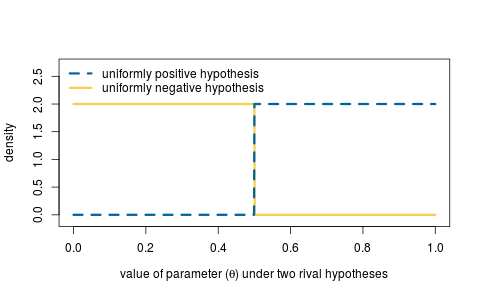
\includegraphics[width=0.49\textwidth]{signed-p.png}\\
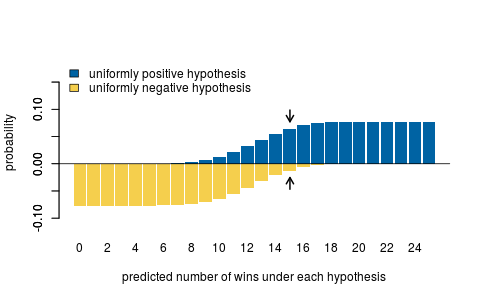
\includegraphics[width=0.49\textwidth]{signed-d.png}
\caption{\textbf{Top.} The representation of the two complementary directional hypotheses. \textbf{Bottom.} The predictions from the models, which look quite different and allow for faster accumulation of evidence.}\label{fig:s}
\end{figure}

The directional comparison is displayed in Figure~\ref{fig:s}.  Note that, due to the way these hypotheses are clearly separated (in the parameter space, top panel), their predictions are quite different as well. Consequently, comparing directional hypotheses will typically yield stronger discriminative evidence than existence/non-existence hypotheses. However, it is important to keep in mind that a comparison between directional hypotheses does not involve any actual null hypothesis -- in this example, both the \hyp{uniformly negative hypothesis} and the \hyp{uniformly positive hypothesis} assume the existence of some difference.  It is tempting to compare these two alternatives and conclude that, because the \hyp{uniformly positive hypothesis} gains much support, there is evidence for a positive effect and therefore evidence for an effect.  This is patently wrong -- the evidence in this case is only for a positive effect \emph{over a negative effect} and \emph{assuming there is some effect}.\footnote{The confusion between what is tested and what can be concluded, and the resultant impression that one can seemingly conclude whether an effect exists by testing only the sign, is sufficiently common that we recently named it the \emph{paradox of le Cornichonesque}, after a snooty fictional wizard \cite{EtzSI}. It is, of course, not a true paradox, but rather an illusion that is resolved by careful consideration of which hypotheses are under consideration \cite{RouderSI}.} Note especially that this analysis gives zero prior probability to a null effect -- in other words, the analysis assumes some effect and could not conclude anything else. One resolution for this problem is discussed in Box~1.

\paragraph{Other pairwise comparisons} As we hope to have illustrated, hypothesis testing is not limited to a comparison between two particular values (e.g., 50\% vs.\ 60\%).  As in many of the examples above, we can test hypotheses that are statements about \emph{ranges} of parameters (e.g., greater than 0.5, or in some small region).

Because in such models the value of $\theta$ is not exactly given (in statistics such a free parameter is sometimes called a ``nuisance parameter''), outside of the simplest cases they cannot be analyzed with classical statistical methods and a Bayesian approach is required.  Fortunately, in the Bayesian framework these models can be dealt with just like any other: all inferential steps are canonical applications of the calculus of probability.

It is hopefully similarly clear that our short list of possible nulls and alternatives is not exhaustive, but that the only limit to the possible comparisons is the imagination of the analyst, whose primary concern should be to match the statistical hypotheses as best they can to the substantive question at hand.  For example, a possibility we have not discussed is the ``interval-and-slab'' comparison (of which the spike-and-slab is an extreme case). Interval-and-slab comparisons will usually give similar results to those of a spike-and-slab comparison, as long as the null interval is relatively narrow compared to the precision afforded by the data---another instance of the teapot problem (see \citeNP{BergerDelampady1987}).
\begin{tcolorbox}[title=Box~1: Evaluating more than two hypotheses at once,code={\singlespacing}]
Not all inference is binary.  There are many scenarios under which more than two hypotheses are pitted against one another.  One useful example was hinted at in the main text: We might want to compare two directional hypotheses, $\H_+$ and $\H_-$, and a point null hypothesis, $\H_0$, all at once.  Nothing prevents us from doing this -- except perhaps for the fact that we are not accustomed to thinking of evidence for one model over two or more others, and this concept is perhaps somewhat more difficult to communicate.  While we can logically and formally work with concepts such as ``the odds of $\H_0 : (\H_+ \lor \H_-)$,'' (where $\lor$ means ``or'') this is cognitively taxing and a seemingly poor way to communicate.\\[-1ex]

On the other hand, we are quite comfortable talking about probabilities as measures of plausibility. We can use the same predictive probabilities as in Equation~\ref{eq:b} to reallocate plausibility across three or more hypotheses. In the case of $K$ hypotheses $\H_1, \H_2, \ldots, \H_K$, we would traditionally compute the posterior probability of one of them, say $\H_1$, with Bayes' theorem: $$P(\H_1|D) = \frac{P(\H_1)P(D|\H_1)}{P(D)},$$ where $D$ is the observed data and the denominator can be re-written as $$P(D) = P(\H_1)P(D|\H_1)+P(\H_2)P(D|\H_2)+\ldots+P(\H_K)P(D|\H_K).$$ If we divide the numerator and denominator of the right-hand side of Bayes' theorem by $P(D|\H_1)$, the probability of the data given hypothesis $\H_1$ (known as the \textit{likelihood}; see \citeNP{EtzLikelihood}), we obtain the following useful reformulation of Bayes' theorem: 
\begin{align*}
P(\H_1 | D) &= \frac{P(\H_1) \frac{P(D|\H_1)}{P(D|\H_1)} }{P(\H_1)\frac{P(D|\H_1)}{P(D|\H_1)} + P(\H_2) \frac{P(D|\H_2)}{P(D|\H_1)} + \ldots + P(\H_K) \frac{P(D|\H_K)}{P(D|\H_1)}}\\
&= \frac{P(\H_1)}{P(\H_1) + P(\H_2) B_{2:1} + \ldots + P(\H_K) B_{K:1}},
\end{align*}
where $B_{j:i}$ is the Bayes factor of hypothesis $j$ over hypothesis $i$. This formula lets us combine the Bayes factors with prior probabilities to obtain posterior probabilities of every hypothesis in a set of any size.\\[-1ex]

For example, suppose that the data we observe are 15 wins in 25 attempts, and we consider $\H_0$, $\H_+$, and $\H_-$.  Following calculations that are given in Box~2, $P(k|\H_0) = 9.74\%$, $P(k|\H_-) = 1.26\%$, and $P(k|\H_+) = 6.43\%$.  Consequently, by taking the ratios of these, $B_{0:-}=7.73$, $B_{0:+}=1.51$, and $B_{+:-}=5.10$.  If we say that $P(\H_0) = 50\%$, $P(\H_+) = 25\%$, and $P(\H_-) = 25\%$, then we can combine these with the Bayes factors to obtain $P(\H_0 | D) = 71.7\%$, $P(\H_+ | D) = 23.7\%$ and $P(\H_- | D) = 4.6\%$.  Now we are able to make simultaneous statements about the existence of \emph{some} effect ($28.3\%$) and its direction: if the effect exists, the probability that it is positive is $23.7/(23.7+4.6) = 83.7\%$.
\end{tcolorbox}
\section*{Summary}
We have focused on one oddly neglected aspect of hypothesis testing: the hypotheses themselves.  It is important to keep in mind that while statistical models are only ever surrogates for our scientific theories, they are the models actually being tested and it is critical that the statistical models we use accurately capture our substantive theories about the data at hand \cite<see also>{rouder2017theories,Vanpaemel:2010}.

We have illustrated with examples that different research questions translate into different formal models, and that the evidence for or against an effect can differ, depending on precisely what is meant by ``no effect.'' However, once this translation from a creative scientific theory to a bespoke statistical model is done, the Bayesian machinery turns and an answer rolls out: We can evaluate the predictive ability of any well-formulated model, and hypotheses that predict the observed data gain plausibility, while hypotheses that do not predict the observed data lose it. {The Bayes factor acts as an automatic Occam's Razor, penalizing vague hypotheses and rewarding precise predictions.} If the observed data are more consistent with the chosen particularization of ``null effect'' than with the chosen particularization of ``some effect,'' then our belief in the null rationally grows.

\section*{R code and the Build-A-Bayes app}

Accompanying this paper is an online demonstration, available via \osf. In the app, users can choose from a selection of pairwise comparisons and change the data and additional model specifications. This allows readers to interactively experience the effects of changes in model specification, which can be large (for example when moving from a spike-and-slab comparison to a directional test) or surprisingly small (for example when moving from a narrow region of negligible-effect to a point null hypothesis).  Additionally, \citeA{Rouder:2016a} also provides a similar development in a blog post titled, ``Roll Your Own: How to Compute Bayes Factors for Your Priors.'' In this blog post, R code is provided to compute Bayes factor in a one-sample design for any hypothesis.

\section*{Discussion and recommendations}

Scientists are tasked with the difficult job of formulating the appropriate scientific question for their context and needs. Once this job is complete, and the scientific question has been translated into an appropriate statistical model, Bayesian methods allow us to compute the evidence for or against a potential claim.

Two steps in this procedure are challenging especially.  First, there is the mapping of a substantive question to a formal model \cite{LeeSI,MatzkeSI,LeeWagenmakersBayesBook,lee2018bayesian}.  This requires expertise, judgment, and a measure of artfulness.  Second, there is the computation of the Bayes factor itself.  For many common cases, researchers are now building and publishing easy-to-use software (e.g., \url{jasp-stats.org}, \citeNP{WagenmakersSI,LoveSI}, and BayesFactor, \citeNP{MoreyRouderBayesFactorPackage}).  However, it will never be the case that all scientific questions will be well addressed by a small set of pre-defined models.  To account for this, others are producing more generic tools and tutorials \cite{gronau2018bridge,MatzkeSI,vanravenzwaaijSI}.\\

\noindent The meteoric rise of Bayesian methods in the social sciences is heartening.  The recent crisis of confidence in psychology has amplified calls for more powerful and flexible methods---including those with the ability to gather evidence for the nonexistence of an effect---and Bayesian inference is ideally suited for this challenge.  But flexibility and power come at a price: the more flexible a tool is, the more extensive its user guide must be. With Bayesian methods, researchers can test any hypothesis they can sufficiently specify.  However, each test carries with it potentially unique implementation (i.e., computational) challenges.  Here we have illustrated methods for testing the null for the simplest possible type of data (binary choice).
However, these methods are universal -- they apply to all sets of hypotheses and models that are sufficiently quantified to make predictions about the data.

The implementation of useful tests and interesting models remains an active field of research and development \cite<e.g.,>{haaf2017developing,OraveczSI}.  The main challenge in this is specifying models that accurately capture theoretical positions.  It is incumbent on researchers to specify such models, justify them, and understand how much our particular specification affects our conclusions.  These activities are, in our opinion, how analysts add value in uncovering the structure in data \cite{Rouder:etal:2016b}.  Model specification is a creative, nuanced, intellectual activity that relies on scientists' substantive expertise.  We believe that the field of psychology is up to this challenge.


\begin{tcolorbox}[title=Box~2: Model definitions and equations,code={\singlespacing}]
For the purposes of statistical inference, a model is defined in sufficient detail if we can compute its predictive distribution $P(\text{data}|\H)$.  In our ESP example, the data are the number of wins $k$ in a sequence of $n$ trials, so that the predictive distribution is more precisely $P_n(k|\H)$.\\[-1ex]

The predictive distribution describes the relationship between the model and the data.  Determining it is a matter of combining the relationship between the model and the parameter (i.e., the prior) with the relationship between the parameter and the data (i.e., the likelihood). Per the sum rule of probability, $P_n(k|\H) = \int_0^1 P(\theta|\H) P_n(k|\theta) \diff\theta.$\\[-1ex]

Both components here are known.  Since the data are a number of wins, the likelihood is a Bernoulli distribution: $$P_n(k|\theta) = \bino{\theta}.$$ The prior is unique to each model, and is given in the table below alongside the predictive distribution of each model and the amount of support at the observed data from the toy example (15 wins out of 25). These calculations and their background are covered more in-depth in \citeA{EtzSI}.\\

\tiny\centering\begin{tabular}{lllr}\hline
Name & Prior $p(\theta|\H)$  & Predictive distribution $P_n(k|\H)$&$P_{25}(15|\H)$\\[1ex]\hline
\hyp{\textbf{point null hypothesis}} 
		& $\H_0:\,\theta = 0.5$                        
		& $\bino{0.5}$ 
		& $.0974$
		\\[1ex]
\hyp{\textbf{competing-point hypothesis}}
		& $\H_A:\,\theta = 0.53$
		& $\bino{0.53}$ 
		& $.1257$
		\\[1ex]
\hyp{\textbf{uniformly positive hypothesis}}
		& $\H_+:\,p(\theta) = u(\theta|0.5, 1.0)$            
		& $\int_0^1 u(\theta|0.5, 1.0) \bino{\theta} \diff\theta$ 
		& $.0643$
		\\[1ex]
\hyp{\textbf{uniformly negative hypothesis}}
		& $\H_-:\,p(\theta) = u(\theta|0.0, 0.5)$
		& $\int_0^1 u(\theta|0.0, 0.5) \bino{\theta} \diff\theta$
		& $.0126$
		\\[1ex]
\hyp{\textbf{negligible-effect hypothesis}} 
		& $\H_N:\,p(\theta) = u(\theta|0.47, 0.53)$ 
		& $\int_0^1 u(\theta|0.47, 0.53) \bino{\theta} \diff\theta$
		& $.0974$
		\\[1ex]
\hyp{\textbf{non-negligible-effect hypothesis}}
		& $\H_L:\,p(\theta) = 0.5 \times u(\theta|0.0, 0.47)$ 
		& $\int_0^1 0.5\left[u(\theta|0.0, 0.47) + u(\theta|0.53, 1.0)\right]$\\
		& $\qquad{+}{\,}0.5 \times u(\theta|0.53, 1.0)$
		& $\qquad\qquad\qquad \times \bino{\theta} \diff\theta$ 
		& $.0694$
		\\[1ex]
\hyp{\textbf{slab hypothesis}} 
		& $\H_S:\,p(\theta) = u(\theta|0.0, 1.0)$
		& $\int_0^1 u(\theta|0.0, 1.0) \bino{\theta} \diff\theta$
		& $.0385$
		\\[1ex]\hline
\end{tabular}\\
\indent\flushleft\small $u(\theta|a,b)$ indicates the uniform probability density between $a$ and $b$, evaluated at $\theta$.
\end{tcolorbox}


\begin{tcolorbox}[title=Box~3: Transitivity of the Bayes factor,code={\singlespacing}]
The Bayes factor has a convenient property known as \textit{transitivity}:  If we have the Bayes factor between $\H_1$ and $\H_2$, $$B_{1:2}=\frac{P(\text{data}|\H_1)}{P(\text{data}|\H_2)},$$ and the Bayes factor between $\H_2$ and $\H_3$, $$B_{2:3}=\frac{P(\text{data}|\H_2)}{P(\text{data}|\H_3)},$$ then the product of $B_{1:2}$ and $B_{2:3}$ gives us 
\begin{eqnarray*}B_{1:2}\times B_{2:3}
&=& \frac{P(\text{data}|\H_1)}{P(\text{data}|\H_2)}\times\frac{P(\text{data}|\H_2)}{P(\text{data}|\H_3)}\\
&=& \frac{P(\text{data}|\H_1)}{P(\text{data}|\H_3)}\\ &=& B_{1:3}~.
\end{eqnarray*}
That is, the Bayes factor between hypothesis $i$ and hypothesis $j$ can be obtained from their respective pairwise Bayes factors with a common comparison hypothesis $k$. This property is often useful when multiple models are compared to one reference model, such as in the case of Bayesian ANOVA \cite{RouderEtAl2012ANOVA}.
\end{tcolorbox}


\bibliography{references}\null

%\newpage\begin{figure}\centering\includegraphics[scale=0.3]{pics/sweep.jpg}\\\large ``Nulls, nulls, nulls...''\end{figure}
\end{document}
